% FIXME: Stick to a naming convention, and disambiguate!
% Resolve:
% - pseudometabolite/bulk metabolite/biomass component/macromolecule
%   --> biomass component metabolite (some aren't macromolecules, e.g. ions)
% - pseudoreaction/isa reaction
%   --> isa reaction (pseudoreaction is too broad, isa reaction introduced in Yeast5),
%   then use biomass component-generating isa reaction
% - biomass reaction/growth reaction/objective function
%   --> prefer biomass reaction
% - use of the term 'flux', esp. 'flux through reaction'
% FIXME: Units/SI units, format them correctly (e.g. mmol gDW-1 h-1)
% and do not use slash characters.
% FIXME: Check if g/mol units for molecular weights of biomass makes sense
% (should it be g/mmol?)
\chapter{Modelling the yeast metabolic cycle}
\label{ch:model}

Discuss difficulty of having a fine-grained model: too many unknowns with this biological system.
Especially that we don't know much about the molecular mechanisms (link to introduction) and the main read-outs of single-cell studies (NAD(P)H, flavins) are `aggregate' measures of enzymatic activity and realistically only function to monitor the cellular redox state.

So what we can only do are coarse-grained models or `coarser' ways to answer biological questions with the YMC.
Here, I present using genome-scale metabolic models and flux balance analysis (FBA) to address the logic of the metabolic cycle --
specifically, why is it advantageous for the cell, and is there a link with resource allocation?

\section{Flux balance analysis}
\label{sec:model-fba}

TODO: Short introduction to genome-scale metabolic models -- what they are, what they aim to do, flux balance analysis, and limitations.

\section{Modelling temporal partitioning of biosynthesis}
\label{sec:model-temporal}
Research question: Given a finite amount of enzymes and the nutrient conditions yeast cells are subject to, is it more efficient for the cells to temporally partition synthesis of macromolecules (lipid, carbohydrates, amino acids), or to synthesise all of them at the same time?
If so, does the time scale fit with that of the yeast metabolic cycle?

There have been studies that attempt to address differing metabolic requirements in each phase of the yeast metabolic cycle using flux balance analysis (FBA).
\textcite{takhaveevTemporalSegregationBiosynthetic2023} showed that in different stages of the cell division cycle, the level of synthesis of each class of macromolecule is different.
They used single-cell NAD(P)H responses (metabolic cycles) to inhibitors that block synthesis of each class of macromolecule to infer the activity of biosynthesis of classes of macromolecules over a cell division cycle.
Then, they used these activities as coefficients for FBA on a modified thermodynamic-stoichiometric metabolic model at each time point to deduce biomass production rates.
% Does not suggest that synthesis of each class of macromolecule excludes all others (which makes sense).
% Rather, this study confirms that timescale of observed synthesis events matches simulations.
% Do I even cite this?  It's so bad.
Additionally, \textcite{cesurGenomeWideAnalysisYeast} constructed a different FBA model for each YMC phase based on transcriptomic and epigenetic data, using the GIMME algorithm, i.e.\ exclude reactions that correspond to genes that are not expressed at certain time points.
Both studies model behaviours at each phase of the YMC, rather than predicting timescale.

An attempt in extending FBA to solve a time-dependent resource allocation problem was \textcite{reimersCellularTradeoffsOptimal2017}, in which they extend a genome-scale model of the cyanobacterium \emph{Synechococcus elongatus} PCC7942 to address the temporal order of intracellular synthesis reactions that optimises the growth rate of the cell, under resource constraints.
However, this model relies on an external oscillation -- namely, the light-dark cycle -- in contrast to the yeast metabolic cycle which is autonomously generated.
Therefore, I can't adapt this to my study.

My approach is to use a genome-scale model of \emph{Saccharomyces cerevisiae} and perform flux balance analysis (FBA).
Specifically, I use the enzyme-constrained Yeast8 (ecYeast8) model \parencite{luConsensusCerevisiaeMetabolic2019}.
I use this model because it is the most recent, offering a good coverage of reactions, and is continuously updated in a well-characterised and well-documented software repository.
Here, I use models Yeast8.6.0 and ecYeast8.6.0, the latest version for which both original and enzyme-constrained variants are available.
In addition, it has `pseudometabolites' defined by \emph{isa} reactions \parencite{heavnerYeastExpandedReconstruction2012} that group specific chemical species in general classes, making it easy to study each class of biomass component (e.g. lipid, protein, carbohydrate) individually.

Traditional genome-scale models assume that the uptake rate of carbon source limits production.
However, levels of each enzyme also restrict reaction fluxes, leading to the development of enzyme-constrained models.
An enzyme-constrained model fits the assumption that there is a fixed number of amino acids the cell has to distribute \parencite{weisseMechanisticLinksCellular2015}.
Models like \textcite{sanchezImprovingPhenotypePredictions2017} and \textcite{elsemmanWholecellModelingYeast2022} -- the latter of which imposes a ribosome capacity constraint and additionally imposes compartment constraints -- constrain the total sum of fluxes based on a defined total amount of enzyme.
ecYeast8 uses the GECKO formalism \parencite{sanchezImprovingPhenotypePredictions2017}, which applies the enzyme constraint by modifying the stoichiometric matrix of a genome-scale metabolic model.

In the next section, I will discuss the formalisms used in ecYeast8 because they differ from the usual formalisms used in other genome-scale metabolic models, and because I take advantage of some of these formalisms.

\section{Yeast8, ecYeast8, and their formalisms}
\label{sec:model-yeast8}

ecYeast8 contains four formalisms relevant to my study:
\begin{enumerate}
  \item
        The biomass reaction is defined by having `pseudometabolites' as reactants and a biomass species as a product.
        These pseudometabolites include lipids, proteins, carbohydrates, RNA, DNA, ions, and cofactors.
        This is in contrast to BiGG genome-scale models that have biomass reactions defined by having chemical species as reactants, each with a stoichiometric coefficient representing the species' abundance in units of mmol gDW-1.
  \item
        The pseudometabolites are defined by `\emph{isa}' reactions, which group specific chemical species into classes of metabolites.
        This accounts for some KEGG definitions of reactions requiring generic compounds and allows flexibility of biomass definition in different growth conditions.
        These \emph{isa} reactions are defined by having chemical species as reactants, each with a stoichiometric coefficient representing the species' abundance in units of mmol gDW-1, and a pseudometabolite as a product.
        In effect, the abundances are shifted one reaction away from the biomass reaction.
  \item
        SLIMEr \parencite{sanchezSLIMErProbingFlexibility2019}, which Splits Lipids Into Measurable Entities, and adds constraints on lipid classes and acyl chain distribution.
        This formalism, specifically for lipid metabolism, is needed because species of lipid backbones and acyl chain can combine to form lipids in more than one thousand ways, and the resulting lipid species are difficult to all be accounted for in a genome-scale metabolic model.
        SLIMEr thus introduces reactions that split lipids into their basic components and lipid pseudoreactions to preserve the distribution of acyl chains.
        The result is that the definitions of lipids are flexible.
  \item
        GECKO was applied to Yeast8 to produce ecYeast8.  GECKO modifies the stochiometric matrix of an input genome-scale metabolic model to account for enzyme abundances and kinetics.
        Specifically, it adds to enzyme-catalysed reactions enzyme species with a stoichiometric coefficient derived from its $k_{cat}$ value.
        The formalism also adds reactions to model drawing enzymes from a pool, with bounds derived from enzyme abundances.  GECKO models the case where there is an upper limit of the amount of amino acids available to be allocated to enzyme production.
\end{enumerate}

Here, I detail how I work around them for my study and take advantage of them.

% FIXME: Delete this subsection?
% It's mostly a duplicate of the appendix of the GECKO paper,
% and I wrote it just to make sure I understand it.
% I haven't used it in discussion so far.
\subsection{GECKO}
\label{subsec:model-yeast8-gecko}

ecYeast8 is derived from Yeast8 by applying the GECKO formalism.
In a conventional genome-scaled model, metabolic fluxes through reactions are constrained between a lower bound and an upper bound.
This is to narrow down the solution space when optimising the objective function.
The GECKO formalism imposes an additional constraint on the metabolic fluxes based on the concentration of the enzyme that catalyses the reaction.
As a simple example, for a reaction $R_{j}$ catalysed by enzyme $E_{i}$ (and $E_{i}$ only), the formalism imposes:

\begin{equation}
  v_{j} \le k_{cat}^{ij} \cdot [E_{i}]
\end{equation}

In other words, the flux through the reaction must not exceed $v_{max}$.
Slightly different relationships are imposed for other types of enzymes, i.e. isozymes, promiscuous enzymes, and enzyme complexes.

To apply this constraint, GECKO modifies reactions in the genome-scaled model it is applied to.
For example, if the model defines a reaction $R_{j}$ catalysed by $E_{i}$:
\begin{equation}
  \ce{ A + B ->[E_{i}] C + D }
\end{equation}

GECKO adds a term to the equation to make it:
\begin{equation}
  \ce{ n_{ij}E_{i} + A + B -> C + D }
\end{equation}
with $n_{ij} = \frac{1}{k_{cat}^{ij}}$.
This transformation, adding the enzyme as a pseudo-reactant, is based on the interpretation that the system uses some amount of enzyme at a specific time to catalyse the flux going through the reaction.

GECKO then also creates an overall enzyme pseudo-reaction $EU_{i}$: $\ce{ -> E_{i}}$, in order to preserve the mass balance of enzymes.  The flux $e_{i}$ of this pseudo-reaction is thus constrained: $0 \le e_{i} \le [E_{i}]$.

Slightly different formalisms are used for reversible reactions, isozymes, promiscuous enzymes, and complexes.  Namely:
\begin{itemize}
  \item Reversible reactions are modelled as the forward and reverse reactions separately.
  \item For isozymes, the original reaction is copied $n$ times and each has as isozyme catalysing the reaction.
  In addition, there is an `arm' reaction to act as an intermediate between the substrate and the products.
  \item No actions are needed for promiscuous enzymes.
  \item Complexes: one reaction that uses all subunit proteins that all share the same $k_{cat}$ value.
\end{itemize}

GECKO repeats this logic for all enzyme-catalysed reactions in the genome-scale model to create an enzyme-constrained model.
GECKO takes $k_{cat}$ values from BRENDA [CITATION NEEDED] and enzyme data from SWISSPROT and KEGG [CITATIONS NEEDED], including molecular weight of protein and associated pathways.
To constrain enzyme levels in the model, GECKO goes through each enzyme and defines upper bounds that correspond to literature values of enzyme properties.
For the proteins that do not have literature values, the constraint is based on the protein mass fraction and a saturation factor.
Then, GECKO scales the amino acid composition so as to reflect the total protein content.
And then changes the carbohydrate composition based on the assumption that a change in the amino acid composition is offset by the reverse change in the carbohydrate composition;
experimental data justifies this assumption.

Alternatively, rather than constraining each enzyme, GECKO can impose a global constraint -- i.e. behave as if none of the proteins have literature values.
GECKO accomplishes this by introducing a pseudo-reaction $ER_{pool}$: $\ce{ -> E_{pool} }$, with a flux $e_{pool} \le (P_{total} - P_{measured}) \cdot f \cdot \sigma$, where $P$ represents protein fraction, $f$ the mass fraction of proteins, and $\sigma$ a parameter that represents the average saturation of enzymes.
And replacing all other pseudo-reactions and replacing them with a global pseudo-reaction $ER_{i}$: $\ce{ MW_{i} E_{pool} -> E_{i} }$.
This approach is similar to FBA with molecular crowding.

The way I use this is just taking ecYeast8.6.0, which assumes the values of the three parameters: $f = 0.5$, $P_{total} = 0.5$, and $\sigma = 0.5$.
These are good first approximations.
This is also a judgement call, especially when the protein fraction varies across growth rates, but $f = 0.5$ is close to the model's mass fraction (insert link to molecular weight calculation section).


\subsection{Computing molecular weights of pseudoreactions}
\label{subsec:model-yeast8-molweights}

In the yeast cell, biomass components (lipids, carbohydrates, proteins) are present in different fractions.
Knowing these fractions are useful in computing the time it takes to synthesise each biomass component (to be discussed later).
However, the mass fraction of each component varies according to strain and growth rate \parencite{nilssonMetabolicTradeoffsYeast2016, elsemmanWholecellModelingYeast2022}, and it is computationally expensive to re-run GECKO each time the protein mass fraction varies.
Therefore, I decided to compute the mass fractions of each biomass component based on the stoichiometries of species in the Yeast8 model, for a back-of-the-envelope calculation.

\emph{isa} reactions define pseudometabolites by having chemical species with known molecular weights as reactants, with their stoichiometric coefficients representing abundance in mmol gDW-1.
Therefore, I can treat each pseudometabolite as a chemical species and calculate its molecular weight by assuming mass balance \parencite{chanStandardizingBiomassReactions2017, dinhQuantifyingPropagationParametric2022, takhaveevTemporalSegregationBiosynthetic2023};
the resulting molecular weight will thus represent the mass fraction of each biomass component in units of g/gDW.

For this to be possible, I needed to compute molecular weights for bulk metabolites that represent macromolecules in the ecYeast8 model.
The ecYeast8 model does not specify the molecular weights of these bulk metabolites.
The bulk metabolites includes: lipids (\texttt{s\_1096}), proteins (\texttt{s\_3717}), carbohydrates (\texttt{s\_3718}), RNA (\texttt{s\_4049}), and DNA (\texttt{s\_3720}).
Additionally, I computed molecular weights for bulk metabolites that represent cofactors (\texttt{s\_4205}), and ions (\texttt{s\_4206}), as they are part of the objective function too.
I applied the procedure that \textcite{takhaveevTemporalSegregationBiosynthetic2023} used to compute the molecular weight of biomass in their model.
Namely, I assumed that in reactions that produce the bulk metabolites, there is conservation of mass, and therefore,

\begin{equation}
\label{eq:conservation-of-mass}
    \sum_{s}(\text{molar mass}_{s})(\text{stoichiometric coefficient}_{s}) - \sum_{p}(\text{molar mass}_{p})(\text{stoichiometric coefficient}_{p})
\end{equation}

where $s = 1, ... (\text{number of substrates})$ represents substrates and $p = 1, ... (\text{number of products})$ represents products of the reaction in question.

This procedure must be applied because the ecYeast8 model does not necessarily imply that each molecule of macromolecule corresponds to a single molecule in a real cell.
Certainly, it is not possible to create a model with such an implication because each species of a macromolecule represented by the bulk metabolite have different molecular weights, and because most macromolecules are polymers -- the model exhibits the average molecular weight of a monomer in such instances.

To compute the molecular weight of the carbohydrate metabolite, I inspected reaction \texttt{r\_4048}:

\texttt{
  0.684535 (1->3)-beta-D-glucan + 0.228715 (1->6)-beta-D-glucan + 0.330522 glycogen + 0.650171 mannan + 0.126456 trehalose \\
  --> carbohydrate
}

Here, the molecular weights of all species except for \texttt{carbohydrate}, the bulk metabolite, are represented in the model.
Thus, equation \ref{eq:conservation-of-mass} can be applied to compute the molecular weight of the carbohydrate metabolite.

The same process can be applied to compute the molecular weights of the DNA, RNA, cofactor, and ion metabolites as the equations similarly have reactants with molecular weights represented in the model and only the bulk metabolite, the sole product, as the metabolite with an unspecified molecular weight.
The DNA molecular weight was computed from reaction \texttt{r\_4050}:

\texttt{
  0.0036 dAMP + 0.0024 dCMP + 0.0024 dGMP + 0.0036 dTMP
  \\ --> DNA
}

The RNA molecular weight was computed from reaction \texttt{r\_4049}:

\texttt{
  0.0445348 AMP + 0.0432762 CMP + 0.0445348 GMP + 0.0579921 UMP
  \\ --> RNA
}

The cofactor molecular weight was computed from reaction \texttt{r\_4598}:

\texttt{
  0.00019 coenzyme A + 1e-05 FAD + 0.00265 NAD + 0.00015 NADH + 0.00057 NADP(+) + 0.0027 NADPH + 0.00099 riboflavin + 1.2e-06 TDP + 6.34e-05 THF + 1e-06 heme a
  \\ --> cofactor
}

And the ion molecular weight was computed from reaction \texttt{r\_4599}:

\texttt{
    3.04e-05 iron(2+) + 0.00363 potassium + 0.00397 sodium + 0.02 sulphate + 0.00129 chloride + 0.00273 Mn(2+) + 0.000748 Zn(2+) + 0.000217 Ca(2+) + 0.00124254 Mg(2+) + 0.000659 Cu(2+)
    \\ --> ion
}

Other metabolites were less straightforward and required some judgement calls.
To compute the molecular weight of the protein metabolite, I inspected reaction \texttt{r\_4047}:

\texttt{
  0.57284 Ala-tRNA(Ala) + 0.200644 Arg-tRNA(Arg) + 0.126979 Asn-tRNA(Asn) + ... + 0.330369 Val-tRNA(Val)
  \\ --> 0.57284 tRNA(Ala) + 0.200644 tRNA(Arg) + 0.126979 tRNA(Asn) + ... + 0.330369 tRNA(Val) + protein
}

In this reaction, the aminoacyl-tRNA reactants are represented in the form of the atoms that make up the aminoacyl residues plus \texttt{R} to represent the tRNA, and the tRNA products are represented as \texttt{RH}.
For example, \texttt{Ala-tRNA(Ala)}, alanyl-tRNA, is represented as \texttt{C3H7NOR}.
The protein pseudoreaction shows how different proportions of each aminoacyl-tRNA combine to form the cell's proteins, so it is safe to discard the \texttt{R} formalism that corresponds to the tRNA from the reaction.
On doing so, the mass balance represented by \ref{eq:conservation-of-mass} can be applied to compute the molecular weight of the protein metabolite.

Finally, the lipid metabolite is the least straightforward because some of the reactants do not have molecular weights specified.
The lipid pseudoreaction is represented in reaction \texttt{r\_2108}:

\texttt{
  lipid backbone + lipid chain --> lipid
}

And both \texttt{lipid backbone} and \texttt{lipid chain} have no molecular weight specified.

Reaction \texttt{r\_4065} specifies a lipid chain pseudoreaction, in which \texttt{lipid chain} is generated:

\texttt{
  0.0073947 C16:0 chain + 0.0217019 C16:1 chain + 0.0020726 C18:0 chain + 0.000796243 C18:1 chain
  \\ --> lipid chain
}

As all reactants have molecular weights defined in the model, the molecular weight of \texttt{lipid chain} can be computed from the mass balance of this reaction.

Reaction \texttt{r\_4063} specifies a lipid backbone pseudoreaction, in which \texttt{lipid backbone} is generated:

\texttt{
  0.000631964 1-phosphatidyl-1D-myo-inositol backbone + 0.00243107 ergosterol + 0.000622407 ergosterol ester backbone + 0.000135359 fatty acid backbone + ...
  \\ --> lipid backbone
}

Within this reaction, all reactants have defined molecular weights except for \texttt{fatty acid backbone}.
Four reactions in the model produce \texttt{fatty acid backbone}.
\begin{table}[ht]
  \centering
    \begin{tabular}{llS}
      ID & Reaction & {\makecell{Computed molecular\\ weight (g/mol)}} \\
      \hline
    \texttt{r\_3975} & \makecell{\texttt{palmitate} \\ \texttt{--> 0.255421 fatty acid backbone + 0.256429 C16:0 chain}} & 742.54 \\
    \texttt{r\_3976} & \makecell{\texttt{palmitoleate} \\ \texttt{--> 0.253405 fatty acid backbone + 0.254413 C16:1 chain}} & 744.56 \\
    \texttt{r\_3977} & \makecell{\texttt{stearate} \\ \texttt{--> 0.283475 fatty acid backbone + 0.284483 C18:0 chain}} & 714.49 \\
    \texttt{r\_3978} & \makecell{\texttt{oleate} \\ \texttt{--> 0.281459 fatty acid backbone + 0.282467 C18:1 chain}} & 716.51 \\
    \end{tabular}
    \caption{ecYeast8 reactions that generate the \texttt{fatty acid backbone} metabolite}
    \label{tab:ecyeast8-fatty-acid-backbone-rxns}
\end{table}

All species in these reactions except for \texttt{fatty acid backbone} have molecular weights specified, and thus I applied mass balance to find the molecular weight of \texttt{fatty acid backbone} from each reaction.
However, the molecular weights computed from each equation are different, as shown in the table above.
Since the differences are slight, and ultimately I am making a back-of-the-envelope calculation, I took the average of the four weights (729.53 g/mol) as the molecular weight of \texttt{fatty acid backbone} for the purposes of computing the molecular weight of \texttt{lipid backbone} (which then yields 21.31 g/mol).

With the molecular weights of \texttt{lipid backbone} and \texttt{lipid chain} defined, I can now compute the molecular weight of \texttt{lipid} using mass balance.

In summary, the molecular weights of the bulk metabolites are:
\begin{table}[ht]
  \centering
  \begin{tabular}{lS}
    Metabolite & {Computed molecular weight (g/mol)} \\
    \hline
    Protein & 504.37 \\
    Carbohydrate & 350.37 \\
    RNA & 64.04 \\
    Lipid & 31.57 \\
    Cofactors & 4.83 \\
    DNA & 3.90 \\
    Ions & 2.48
  \end{tabular}
  \caption{Computed molecular weights of bulk metabolites in ecYeast8}
  \label{tab:ecyeast8-mol-weights}
\end{table}

As additional validation, the ratio between the molecular weights are similar to the ratio between the mass of each class of macromolecule in the yeast cell dry weight shown by Grigiatis [TODO: Add proper citation].

And thus the molecular weight of biomass is 961.57 g/mol, close to the 966 g/mol in \textcite{takhaveevTemporalSegregationBiosynthetic2023} computed from a different genome-scale model.
In theory, this number should be 1000 g/mol because the stoichiometric coefficients of the species that form biomass components are expressed in terms of mmol per gDW \parencite{thieleProtocolGeneratingHighquality2010, palssonSystemsBiologyConstraintbased2015}, but the slight deviation from 1000 could be explained by the SLIMEr formalism;
plus, it has been reported that the sum of stoichiometric coefficients are not always verified \parencite{chanStandardizingBiomassReactions2017}.

% Could move to 'results' part of this chapter?
\subsection{Ablating pseudometabolites from the biomass reaction}
\label{subsec:model-yeast8-pseudometabolites}

I take advantage of the presence of pseudometabolites to remove each of them in turn (easily) from the biomass reaction.

In my approach, I exclude each class of macromolecule in turn in the objective function (biomass-generating reaction) and optimise the model.
Specifically, given the objective function:

\texttt{
  55.3 atp\_c + 55.3 h2o\_c + lipid\_c + protein\_c + carbohydrate\_c + dna\_c + rna\_c + cofactor + ion \\
  --> 55.3 adp\_c + biomass\_c + 55.3 h\_c + 55.3 pi\_c
}

There are five classes of macromolecules: lipids, proteins, carbohydrates, DNA, and RNA.
To have the cell prioritise biosynthesis of lipids, I set the stoichiometries of all five classes except for lipids to zero in the above equation, giving:

\texttt{
  55.3 atp\_c + 55.3 h2o\_c + lipid\_c + cofactor + ion \\
  --> 55.3 adp\_c + biomass\_c + 55.3 h\_c + 55.3 pi\_c
}

And I repeated this for the other four macromolecules.

\section{Exchange reaction saturation}
\label{sec:model-saturation}

For various purposes [INSERT WHICH PURPOSES HERE], I need to know the saturation of the exchange reactions -- i.e. the uptake goes up and up, but at some point the growth rate maxes out.
This follows \textcite{elsemmanWholecellModelingYeast2022}, in which they deal with how FBA doesn't account for concentrations of substrates in the media by varying glucose uptake in the model and see how the growth rate changes, producing a sort of saturation curve that agrees with the theoretical basis of saturation of glucose transporters [TODO: FACT-CHECKING THIS SENTENCE, AND RE-WRITE SO IT IS MORE SCIENTIFIC].

Using the ecYeast8.6.0 model, I varied the flux bounds of exchange reaction and recorded how it affects predicted growth rate.
I did this with two carbon sources to be investigated later, glucose and pyruvate, and with ammonium as a nitrogen source.

[TODO: REMOVE NON-WILD TYPE CURVES]

\begin{center}
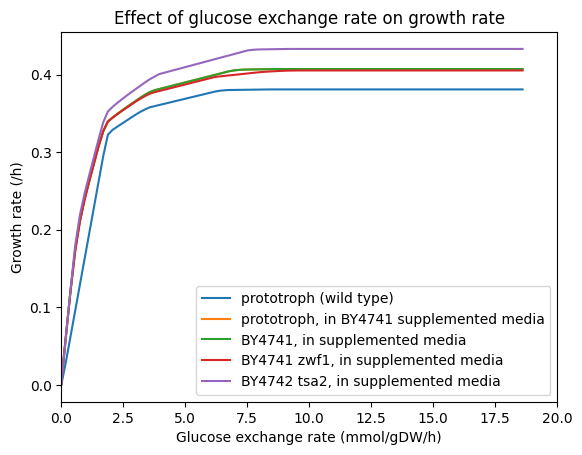
\includegraphics[width=.9\linewidth]{ecYeast8-glucose-saturation.png}
\end{center} Figure X: Glucose saturation

\begin{center}
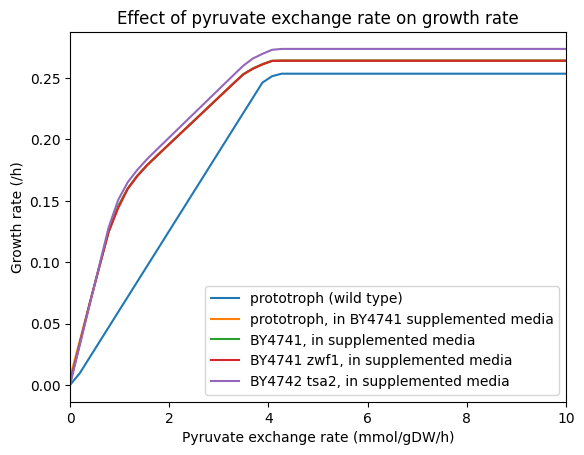
\includegraphics[width=.9\linewidth]{ecYeast8-pyruvate-saturation.png}
\end{center} Figure X: Pyruvate saturation

\begin{center}
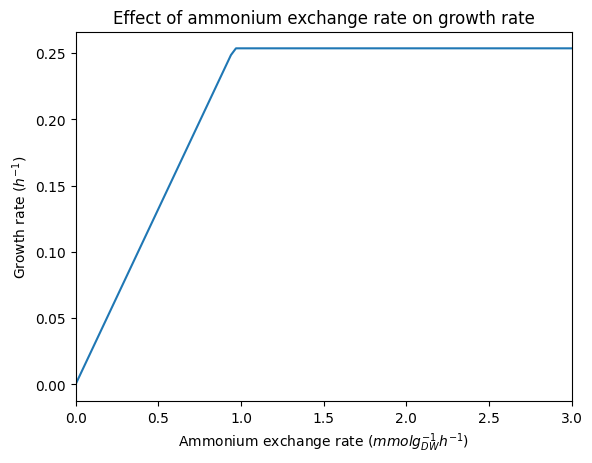
\includegraphics[width=.9\linewidth]{ecYeast8-ammonium-saturation.png}
\end{center} Figure X: Ammonium saturation.  Glucose uptake set to 16.89, optimal found by non-modified model.

% Working title.
% TODO: come up with a better one.
\section{Estimating timescale of biosynthesis}
\label{sec:model-timescale}

I used the ecYeast8.6.0 model with glucose uptake restricted to 0 $\leq$ 16.89 $\leq$, as the optimal value found by the non-modified model.
This value agrees with theoretical saturation rates of 16 $\sim$ 19 mmol gDW-1 h-1.
Using the biomass reaction as the objective function, I optimise the model to obtain the predicted growth rate, and computed the doubling time based on this growth rate as follows:

\begin{equation}
  t = \frac{\ln 2}{\lambda}
\end{equation}

where $t$ is the doubling time and $\lambda$ is the growth rate, equivalent to the optimal flux of the biomass reaction.

I ablate components in biomass reaction (i.e.\ macromolecules like lipids, proteins, carbohydrates, DNA, RNA, and also cofactors \& ions) that have pseudoreactions associated with the 'Growth' subsystem, as discussed in previous section (INSERT LINK HERE) in turn.
In each round, the model is simulated, using the modified biomass reaction as the objective function, and the flux is recorded.
Doubling time is computed, taking into account the mass fraction of each biomass component -- i.e.\ if the component is a smaller fraction of the cell, it takes less time.
Specifically, the computation is:

\begin{equation}
  t_{i} = f_{i} \cdot \frac{\ln 2}{\lambda_{i}^{\prime}}
\end{equation}

where $i$ represents each of the biomass components (lipids, proteins, carbohydrates, DNA, RNA, cofactors, and ions), $t_{i}$ is the predicted time for synthesis of each biomass component, $f_{i}$ is the mass fraction of each biomass component, and $\lambda{i}^{\prime}$ is optimal flux of the ablated biomass reaction.
$f_{i}$ for each biomass component is computed by dividing the molecular weight of the corresponding pseudometabolite by the molecular weight of biomass (see table X -- LINK TO TABLE TO MOLECULAR WEIGHTS).

For comparison, I computed estimates of the time for each biomass component, assuming that it is proportional to the mass fraction [BUT, WHY?]:

\begin{equation}
  t_{i} = f_{i} \cdot t
\end{equation}

where $t$ is the doubling time found in equation X [LINK TO THE FIRST ONE].

[INSERT BAR CHART: SHOWING FLUXES OF ORIGINAL BIOMASS REACTION AND THE SEVEN ABLATED ONES]

\begin{center}
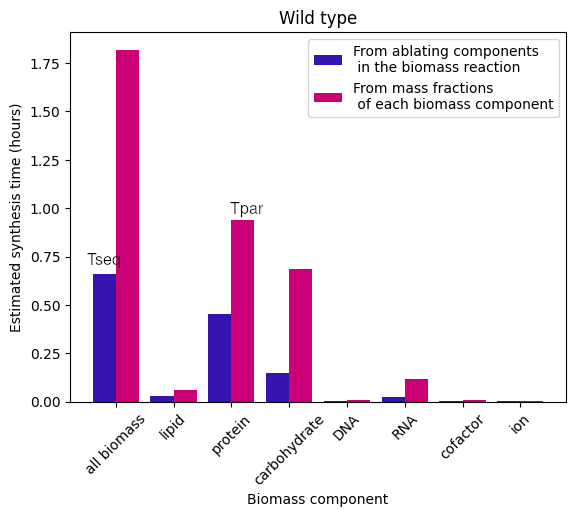
\includegraphics[width=.9\linewidth]{ablation_example_ratio.png}
\end{center} Figure X: Comparing time scales derived from ablating components of the biomass reaction (blue) and from assuming that synthesis time is proportional to the mass fraction of the biomass component (red).  Times for each biomass component (lipid, protein, carbohydrate, DNA, RNA, cofactor, ion) were computed according to equations X--Y.  Blue under `all biomass' is the sum of times derived from ablation (other blue bars), while red under `all biomass' is derived from the flux of the original biomass reaction (equation X).  As a summary value, the ratio between the total time predicted by ablation and the biomass component that is predicted to take the most time is computed (ratio = A/B, as on figure).

And as a summary value, the ratio between the total time predicted by ablation and the biomass component that is predicted to take the most time is computed (ratio = A/B, as on figure).
A represents sum of times from focusing on each biomass component -- thus represents time predicted, assuming biomass components are synthesised in turn.
B represents time of synthesis of protein component if time is assumed to be proportional to mass fraction.
This is always protein as it accounts for $\approx$50\% of the mass fraction.
B thus represents the limiting, slowest process
A smaller A/B ratio (< 1) means that -- under these conditions -- synthesising biomass components in sequence saves more time.
In this case, the ratio is about 0.7.

% ------
% NEXT STEPS:
% - Headline ablation results ('robustness')
The fact that this still holds true for auxotrophs and deletion strains supports experimental evidence that auxotrophs and deletion strains have YMCs.

[INSERT ABLATION BAR CHARTS: BY4741, BY4742, zwf1, tsa2]

% Adding supplements, e.g. amino acids, dNTPs/NTPs, pyruvate, glucose limitation?

% - Heatmap results
% *** Leave this mostly in bullet points for now because the results are WIP/in flux
I aim to assess the effect of carbon and nitrogen source uptake on this ratio.

\begin{center}
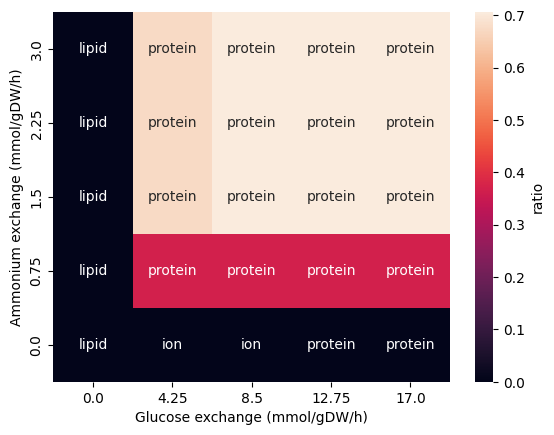
\includegraphics[width=.9\linewidth]{ecYeast8-ablation-heatmap.png}
\end{center}

The ratio maxes out at about 0.7.  The black regions = zero growth, due to zero uptake of C/N -- safe to ignore these.

\begin{center}
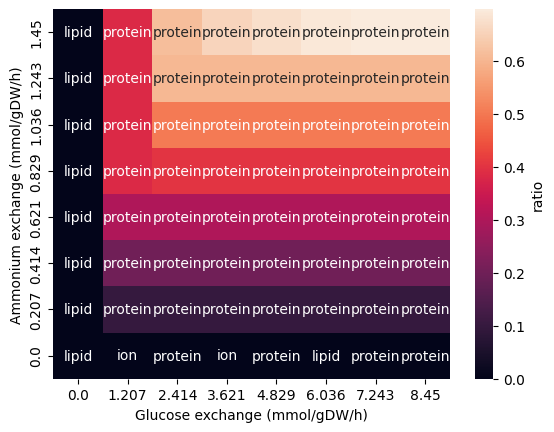
\includegraphics[width=.9\linewidth]{ecYeast8-ablation-heatmap-under_saturation_8x.png}
\end{center}

Zoom in region below saturation: ammonium exchange rates affect the ratio more than glucose.
At e.g.\ glucose saturation, ammonium exchange rate controls the ratio.
If the ammonium exchange rate is low, indicating nitrogen limitation, then the biomass flux is (comparatively) high, and temporal partitioning is more advantageous for the cell.

\begin{center}
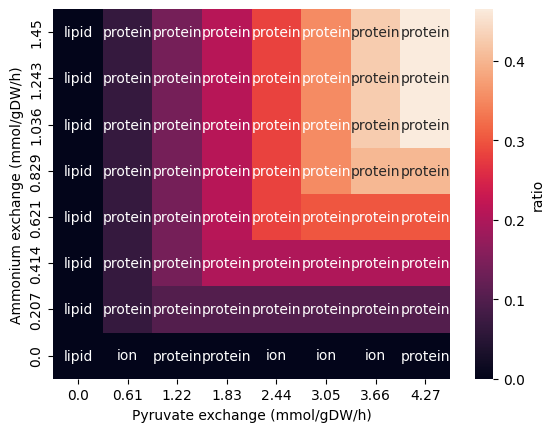
\includegraphics[width=.9\linewidth]{ecYeast8-ablation-heatmap-pyruvate-under_saturation_8x.png}
\end{center}

In contrast, if pyruvate is used as the carbon source, at high ammonium exchange rates, pyruvate seems to be the thing that controls the ratio (which maxes out at about 0.4).
If both are low, there is a combinatorial effect.

Taken together, this suggests that temporal partitioning is a strategy advantageous under growth-limiting conditions, and would explain why YMCs occur in these conditions, including during glucose starvation.


% TODO: Fix conclusion
Therefore, I conclude that given a finite amount of enzymes, it is more efficient to partition synthesis of macromolecules temporally, and the time scale is at the same order of magnitude as the yeast metabolic cycle.

Upon closer inspection of the times and fluxes... [INSERT RESULTS AND DISCUSSION HERE]
% - How long does it take to replicate the genome?  It is biosynthesis of nucleotides + process of polymerising them.  There has to be super basic cell division cycle literature about this...
% - Fatty acids: cell may use pentose phosphate pathawy and gluconeogenesis to route flow in a cycle to generate masses of NAD(P)H.  Check if the fluxes suggest this.

Discussion: Although it is unrealistic to assume that synthesis of one class macromolecule excludes all others, this approach is still instructive as it gives a back-of-the-envelope calculation to support the notion that the cell partitions biosynthesis temporally, and gives weight to the idea that this may be one of the rationale of the existence yeast metabolic cycle.
Furthermore, the timescale gleaned from this investigation may explain the discrepancy between the shorter (on the range of 1 hour) single-cell metabolic cycles and the longer (on the range of 4 hours) dissolved oxygen oscillations in chemostats along with the longer (on the range of 10 hours) cell division cycles in chemostats.
% give some idea of explanation here
From a biochemical perspective, [DISCUSS IMPLICATIONS FROM LOOKING AT FLUXES]

% % AM I STILL DOING THIS??
% \section{Modelling chemostat-based studies}
% \label{sec:model-chemostat}
% % - Metabolic responses to environment
% % - Cell communication
% % - Relating them to the single-cell yeast metabolic cycle

% Cite \textcite{jonesCyberneticModelGrowth1999}.

% \section{Coarse-grained, phenomenological model}
% \label{sec:model-coarse}

% % leads nicely to conclusion
